\begin{figure}
    \centering
    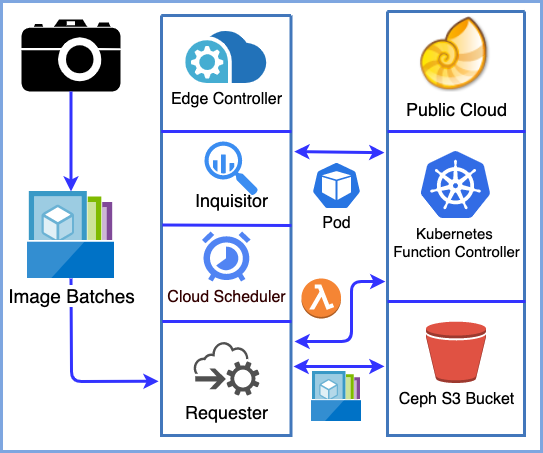
\includegraphics[scale=0.4]{figures/STOIC.png}
    \caption{The STOIC Architecture \label{fig:STOIC}}
\end{figure}

To leverage hardware acceleration and distributed scheduling within a
serverless architecture, we have developed STOIC, a framework for executing
analytics applications in multi-tier IoT (sensing-edge-cloud) settings. STOIC
optimizes the end-to-end process of packaging, transferring, scheduling,
executing, and result retrieval for machine learning applications in and
egde-and-cloud setting.  Figure~\ref{fig:STOIC} shows the distributed
components of STOIC. On an edge device, STOIC gathers application input data,
determines whether the lower application latency will be achieved by
processing the data on the edge or in the cloud, and then actuates the
application's computation (with the necessary data) using the ``best'' choice.
The public cloud component manages what ever cloud resources are needed to
recive the data from the edge, trigger the computation, and to return the
results to the edge.  We have designed the system as a result of a need to
classify wildlife images in a location where it is possible to site a
relatively powerful edge device (a small board computer) but where network
connectivity is poor.  In this paper, we report on its use for processing
images from multiple, motion-triggered camera traps (sensors) deployed to
a wildlife preserve currently used to study ecological land use.
%monitor wildlife across the Sedgwick Natural Reserve~\cite{ref:sedgwick}.

\subsection{Edge Controller} 

The edge controller is a server that runs in an
outbuilding at the reserve. It communicates wirelessly with the sensors and
triggers analysis/computation upon their arrival. The edge controller is
connected to a research facility (which has full Internet connectivity) 
%remove for blind: the UCSB campus
via a microwave link. When a camera trap detects
motion, it takes photos and persists the images in flash storage.
Periodically, the sensors transfer saved photos to the edge controller. Up to
the end of a transfer cycle, edge controller packages all images generated
within this hour and transfers it to the public cloud if necessary when the
tasks are scheduled on it. STOIC runs on the edge controller and its execution
is triggered by the arrival of image batches. 

As an intermediate computational tier between the sensors and the public
cloud, the edge controller can be placed anywhere, preferably near the edge
devices, to lower the response latency for the data processing and analytics
applications. It consists of three major components: 
\begin{itemize}
\item The \textbf{cloud
scheduler} predicts the total latency based on historical data in a local
database for each available runtime. 
\item The \textbf{requester} firstly
dispatches the image batch to a dedicated Ceph~\cite{ref:ceph} S3 bucket when
the workload is scheduled at the public cloud, secondly deploys the runtime
having the least latency and triggers the  serverless function via a
RESTful HTTP request either locally at the edge cloud or remotely in the
public cloud. 
\item The \textbf{inquisitor} constantly deploys all runtimes as
Kubernetes pods~\cite{ref:pods} and records the deployment time respectively
in the database. We use the inquisitor to establish the time series for
predicting deployment latency.
\end{itemize}

The edge cloud that we use in this study is deployed in our lab on campus,
which is connected to both the reserve and the Internet. It consists of a
cluster of nine Intel NUCs~\cite{ref:nucs} (6i7KYK), each with two Intel Core
i7-6770HQ 4-core processors (6M Cache, 2.60 GHz) and 32GB of DDR4-2133+ RAM
connected via two channels. The cluster is managed using the Eucalyptus cloud
system~\cite{ref:euca}, which mirrors the Amazon Web Services (AWS) interfaces
for Elastic Compute Cloud (EC2) to host Linux virtual machine instances and
Simple Storage Service (S3) to provide object storage.
 
\subsection{Public/Private Cloud}

To investigate the use of the serverless architecture with hardware
accelerators, we employ a shared, multiuniversity, GPU cloud, called
Nautilus~\cite{ref:nautilus}, as our remote cloud system. Nautilus is an
Internet-connected, HyperCluster research platform developed by researchers at
UC San Diego, the National Science Foundation, the Department of Energy, and
multiple, participating universities globally.  Nautilus is designed for
running data and computationally intensive applications and uses
Kubernetes~\cite{ref:k8s} to manage and scale containerized applications. It
also uses Rook~\cite{ref:rook} to integrate Ceph for data storage. As of May
2020, Nautilus consists of 176 computing nodes across the US and a total of
543 GPUs in the cluster. All nodes are connected via a multi-campus network.
In this study, we consider Nautilus as a public cloud that enables us to
leverage hardware acceleration (GPUs) in the serverless architecture to serve
edge devices. 

One major challenge we face with such deployments is hardware heterogeneity
and performance variability. On Nautilus, we have observed 44 different types
of CPU (e.g. Intel Xeon, AMD EPYC, among others) and 9 GPU types (e.g. Nvidia
1080Ti, K40, etc.). Both CPUs and GPUs of different types have different
performance characteristics. Besides, ceph storage is run on dedicated nodes
that distributed globally.

This heterogeneity impacts application execution time (which STOIC attempts to
predict) in three significant ways. First, different CPU clock rates affect
the transfer of datasets from the main memory to GPU memory. Second, there is
significant latency and variable performance between runtimes and the storage
service (which hold the datasets and models). Third, the multi-tenancy of
nodes (common in public cloud settings) allows other jobs to share
computational resources with our applications of interest at runtime. 

These three factors negatively affect our goal of designing STOIC, which is to
efficiently execute IoT applications with minimum latency. With STOIC, we
address these challenges to build a novel scheduling system that adapts to
this variability. Moreover, to reduce heterogeneity and ensure repeatability
of our results, we confine nodes and GPUs to a single Nautilus region.
%we use node affinity~\cite{ref:nodeAffinity} to confine the nodes only in the
%UCSD region. This configuration effectively reduces the heterogeneity of the
%cluster and ensure the reliability of the following experiments.

\subsection{Runtime Scenarios}

To schedule machine learning tasks across hybrid cloud deployments, we define
four runtime scenarios: \textbf{(A)} \textit{edge} - A VM instance on the edge
cloud with AVX2~\cite{ref:avx} support; \textbf{(B)} \textit{cpu} - A
Kubernetes pod on Nautilus containing a single CPU with AVX2~\cite{ref:avx}
support; \textbf{(C)} \textit{gpu1} - A Kubernetes pod on Nautilus containing
a single GPU; \textbf{(D)} \textit{gpu2} - A Kubernetes pod on Nautilus
containing two GPUs.  STOIC considers each of these deployment options as part
of its scheduling decisions. Users can parameterize STOIC with their choice of
deployment or allow STOIC to automatically schedule their applications.


\subsection{Execution Time Estimation}

As depicted in Figure~\ref{fig:STOIC}, the STOIC socket client executes in the
edge cloud and listens for requests from the edge controller (machine learning
job requests). After a preset period (parameterizable but currently set to an
hour), STOIC estimates total response time~($T_s$) of a requested batch, based
on 4 different runtime scenarios. The total response time ($T_s$) includes
data transfer time~($T_t$), runtime deployment time~($T_d$) and the
corresponding processing time~($T_p$). We define total response time~($T_s$)
as $T_s = T_t + T_d + T_p$.
 
\subsubsection{Transfer time ($T_t$)} 

$T_t$ measures the time spent in transmitting a compressed batch of images
from the edge controller to edge cloud and public cloud.  We calculate
transfer time as ${T_t = F_b / B_c}$ where $F_b$ represents the file size of
batch and $B_c$ represents the bandwidth at the moment provided by a bandwidth
monitor at the edge controller. 
 
\subsubsection{Runtime deployment time ($T_d$)} 

$T_d$ measures the time
Nautilus uses to deploy requested kubeless function. Since the scarcity of
computation, it is common that multi-GPU runtime takes longer to deploy than
single-GPU and CPU runtimes. Note that, for \textit{edge} runtime, the
deployment time zeroes out since STOIC executes the task locally in the edge
cloud.
 
\begin{figure*}
    \centering
    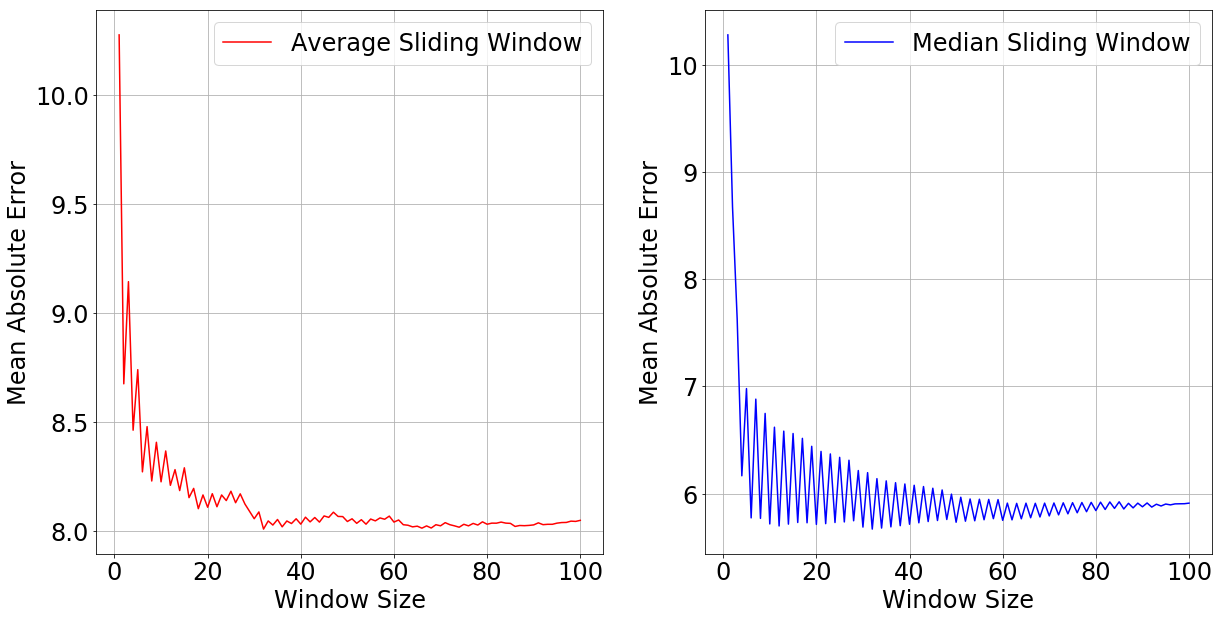
\includegraphics[scale=0.3]{figures/deployment}
    \caption{The Mean Absolute Error (MAE) of deployment time for the \textit{gpu1} runtime. The x-axis is window (history) size. The left subplot is MAE when STOIC uses average sliding window, the right subplot is MAE when STOIC uses median sliding window.
\label{fig:deployment}}
\end{figure*}

 
\begin{table}
\centering
\scriptsize
\resizebox{\columnwidth}{!}{
\begin{tabular}{|c|c|c|c|} 
\hline
& & \textbf{Optimal} & \textbf{Minimum}  \\
\textbf{Modeling} & \textbf{Runtime} & \textbf{Window Size} & \textbf{MAE}  \\
\hline
AutoReg & cpu & 15 & 8.977 \\
\hline
AutoReg & gpu1 & 15 & 9.605 \\
\hline
AutoReg & gpu2 & 15 & 17.918 \\
\Xhline{2\arrayrulewidth}
Avg. SW & cpu & 33 & 7.714 \\
\hline
Avg. SW & gpu1 & 31 & 8.006 \\
\hline
Avg. SW & gpu2 & 91 & 16.52 \\
\Xhline{2\arrayrulewidth}
Med. SW & cpu & 13 & \textbf{5.96} \\
\hline
Med. SW & gpu1 & 31 & \textbf{5.668} \\
\hline
Med. SW & gpu2 & 27 & \textbf{14.48} \\
\hline
\end{tabular}
}

\caption{Mean Absolute Error for three time series modeling methods: auto-regression (AutoReg), average sliding window (Avg. SW), and median sliding window (Med. SW). Median sliding window achieves the lowest minimum MAE at optimal window size (that with the lease MAE) for all three runtimes. \label{tab:deployment}}
\end{table}
 

We observe significant variation in deployment time on Nautilus for different
times of the day. To accurately predict deployment time, we analyze deployment
times as a time series using three methods: (1) auto-regression modeling, (2)
average sliding window, and (3) median sliding window.
Auto-regression~\cite{ref:autoreg} is a time series modeling technique based
on the auto-correlation between previous time steps and following ones.
Average sliding window is the moving average~\cite{ref:moveavg} scanning
through the time series by a fixed-length window. Similarly, the median
sliding window is the moving median throughout the time series. All the window
sizes used for three modeling processes are optimized based on historical data
of deployment time~($T_d$) in January, 2020. We then compare the minimum Mean
Absolute Error (MAE) from each to select the best modeling methodology. 

We consider a time series of 1244 data points for each runtime.
Figure~\ref{fig:deployment} shows representative analytics for \textit{gpu1}
deployment time, in which MAE oscillates as window size varies. We observe
that the median sliding window reaches lower minimum MAE than average sliding
window at optimal window size. As listed in Table~\ref{tab:deployment}, all
three runtimes achieve the lowest minimum MAE using median sliding window.
Therefore, STOIC adopts this methodology for deployment time prediction. 

To form a control-loop feedback mechanism, STOIC constantly calibrates the
optimal sliding window size while executing, based on the most current
deployment time series logged by the inquisitor. The number of data points
used in analytics (i.e. 100 by default) and the interval of calibration (i.e.
every 10 executions by default) are both parameterizable, in the consideration
of tuning between performance and accuracy. 
 
\subsubsection{Processing time~($T_p$)} 

$T_p$ is the execution time of a
specific machine learning task and the target of task scheduling across the
hybrid cloud. STOIC formulates a linear regression on execution time histories
and uses it to predict processing time, based on the batch size. Specifically,
we use Bayesian Ridge Regression~\cite{ref:brr} due to its robustness to
ill-posed problems (relative to ordinary least squares
regression~\cite{ref:ols}). STOIC queries the database for the most recent
processing time data (e.g. 10 data points) for each regression. This ensures
that the parameters of the regression line reflect the current runtime
performance.
 
As part of our investigations into this approach, we have found that this
approach is highly susceptible to outliers. The root cause is sporadic
congestion and maintenance (for nodes, networking, etc.) of the public cloud.
Deviating significantly from the average, outliers skew the regression line
and overestimate the runtime latency for extended periods of time (due to the
windowing approach). We thus update the regression using a random sample
consensus (RANSAC) technique~\cite{ref:ransac}, which iteratively removes
outliers from the regression. The algorithm~\ref{algo:ransac} illustrates the
implemented RANSAC approach.

\begin{algorithm}[]
\caption{Random Sample Consensus}
\label{algo:ransac}
\SetAlgoLined
\KwData{
(1) Observation set of Process time $T_p$\\
(2) Bayesian Ridge Regression model $M$\\
(3) Minimum sample size $n$\\
(4) Residual threshold $t$\\
(5) Maximum iteration $k$ \\
(6) Required inliner size $d$ \\ 
(7) Minimum Root Mean Square Error $e$ \\
}
\KwResult{A set of parameters that best fits the data}
 \While{iterations $\leq$ k}{
    curr\_sample := $n$ data points from observation\;
    curr\_model := $M$ regressed on curr\_sample\;
    fit\_data := empty set\;
    \For{ every data point $p$ in curr\_sample}{
        \uIf{error of $p$ $\leq$ $t$}{
            $p$ $\to$ fit\_data\;
        }
    }
    \eIf{fit\_data size $\geq$ $d$}{
        \uIf{curr\_error < $e$}{
            Update $M$ and $e$
        }
    }{Increment iteration}
 }
 return $M$
\end{algorithm}
 
 \begin{figure*}
    \centering
    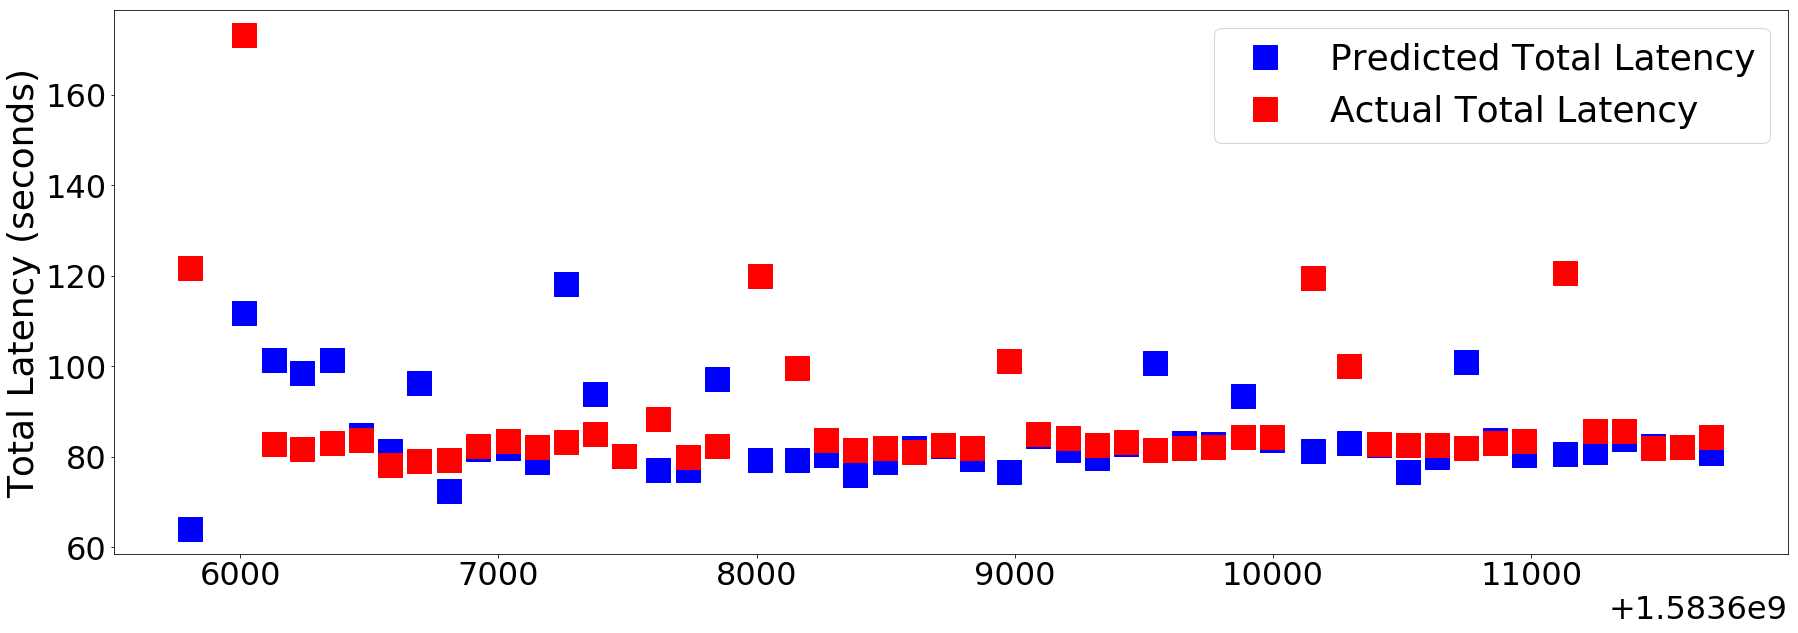
\includegraphics[scale=0.20]{figures/timeline.png}
    \caption{The comparison of predicted and actual total latency on 50 \textit{gpu1} benchmark executions with 150-image batch size. The x-axis is the epoch time and the y-axis is the total latency. \label{fig:timeline}}
\end{figure*}

\begin{table}
\centering
\scriptsize
\resizebox{\columnwidth}{!}{
\begin{tabular}{|c|c|c|c|} 
\hline
 & \textbf{Deployment $T_d$} & \textbf{Processing $T_p$} & \textbf{Total $T_s$}  \\
\hline
First Half & 42.7\% & 11.2\% & 15.8\% \\
\hline
Second Half & 29.2\% & 5.3\% & 9.2\% \\
\hline
\end{tabular}
}

\caption{The percentage mean absolute error (PMAE) of deployment, processing and total latency.  \label{tab:timeline}}
\end{table}
 
 \subsubsection{Adaptability}
 
To verify that STOIC's estimation of execution time captures the actual
latency of the public cloud, we repeatedly execute our application 50 times
with 150-image batch using the \textit{gpu1} runtime. Depicted in
Figure~\ref{fig:timeline}, we observe that actual total latency varies
significantly and predicted total latency has a non-negligible difference from
the actual total latency at the beginning of the experiment. However, over
time, as STOIC learns the various latencies of the system, the difference is
significantly reduced. In Table~\ref{tab:timeline}, we report the percentage
mean absolute error (PMAE), which we compute as the MAE divided by mean
latency. The decrease in all three PMAE values in the second half of the
execution trace also shows STOIC's adaptability.

\begin{figure*}
\centering
\begin{minipage}{.50\textwidth}
  \centering
  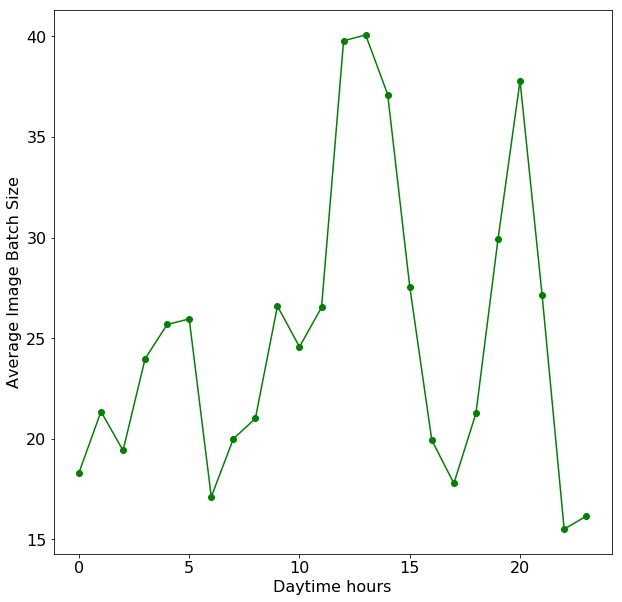
\includegraphics[width=\linewidth]{figures/Hourly_act.png}
  \captionof{figure}{Wildlife Hourly Activity Level. The figure demonstrates the mean activity level of wildlife throughout a day. Based on the curve, 1PM and 8PM are two peak hours of animal activities.}
  \label{fig:hour_act}
\end{minipage}%
\begin{minipage}{.50\textwidth}
  \centering
  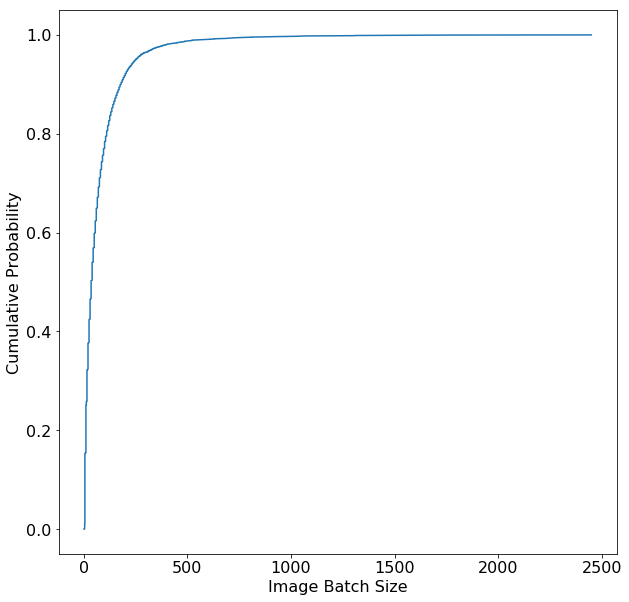
\includegraphics[width=\linewidth]{figures/ecdf.png}
  \captionof{figure}{Conditional Empirical Cumulative Distribution Function. The STOIC image batch simulator is based on this function and random probabilities [0, 1) from a uniform distribution.}
  \label{fig:cdft}
\end{minipage}
\end{figure*}

%\begin{figure}[t] \centering 
%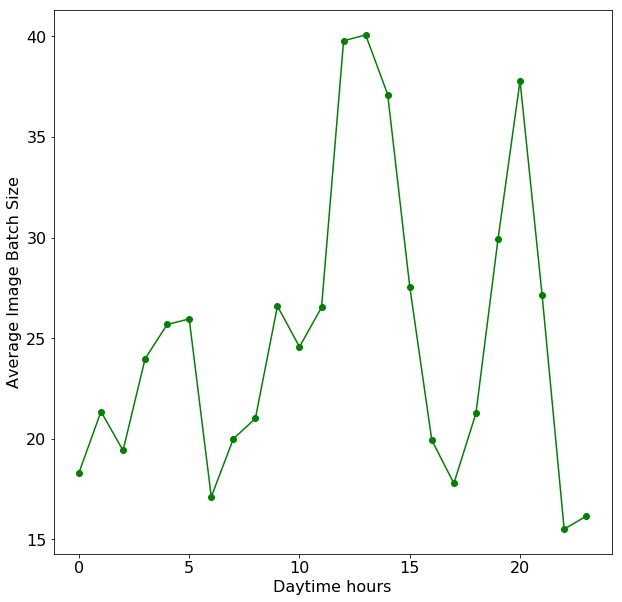
\includegraphics[scale=0.36]{figures/Hourly_act.png}
%\caption{Wildlife Hourly Activity Level. The figure demonstrates the mean activity level of wildlife throughout a day. Based on the curve, 1PM and 8PM are two peak hours of animal activities.
%\label{fig:hour_act}}
%\end{figure} 
 
 
%\begin{figure}[t] \centering 
%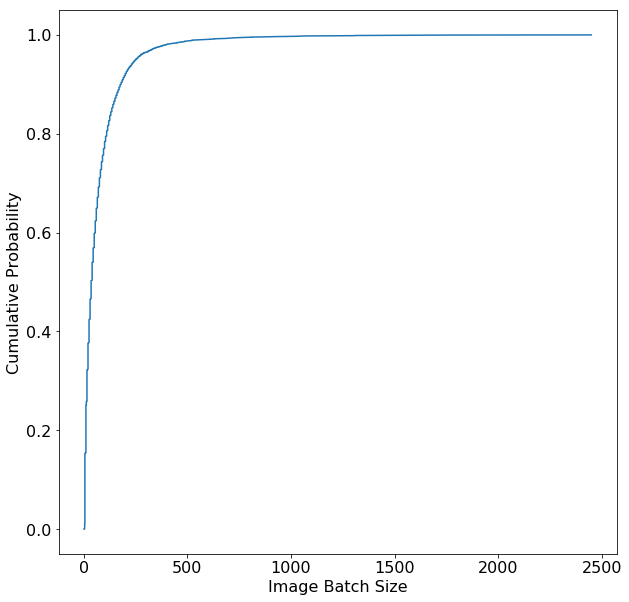
\includegraphics[scale=0.36]{figures/ecdf.png}
%\caption{Conditional Empirical Cumulative Distribution Function. The STOIC image batch simulator is based on this function and random probabilities [0, 1) from a uniform distribution.
%\label{fig:cecdf}}
%\end{figure} 
 
\subsection{Simulator}

Since the network infrastructure was under construction at Sedgwick natural
reserve when we built up STOIC, we created a simulator that mimics the
generation of image batches from camera traps. First, we obtain a set of
motion-detected images from July 13th, 2013 to Jan. 15th, 2017. After
excluding maintenance days in between, we process 1136 effective days (27264
hours) of data. The maximum size of hourly image batch is 2450, whereas the
minimum size is unsurprisingly zero, which constitute 18139 hours out of 27264
hours (66.53\%). On average, the hourly image batch size is 25.
Figure~\ref{fig:hour_act} illustrates the wildlife hourly activity level based
on the image batch size. We infer from the curve that 1PM and 8PM are two peak
hours of animal activities during daytime. 

To simulate the generation of image batches from camera traps, we construct an
conditional empirical cumulative distribution function~(ECDF) based on
probability definition of  $Pr(x < K | x > 0)$, where x is the image batch
size and K is the cutoff value. This conditional ECDF effectively represents
the trajectory of animal activity level and makes the evaluation empirical.
Figure~\ref{ref:cecdf} plots the conditional ECDF. The x-axis is the image
batch size ranging from zero to 2450, whereas the y-axis is the cumulative
probability. The sampling procedure is as follows.  During the execution of STOIC, the simulator first generates a
random number in [0, 1) from a uniform distribution and secondly retrieves the
corresponding image batch size from the conditional ECDF. Using this process,
we are able to evaluate and draw conclusions by replaying the image stream
from the camera traps in fast-than-real time for the purposes of comparative
evaluation.
%, regarding STOIC's
%performance and efficiency by a real-world streaming data flow.



 \subsection{Implementation}

Considering performance and interface, we implement STOIC using
Golang~\cite{ref:golang}. Golang provides high performance execution (vs
scripting languages) and a user-friendly interface~\cite{ref:client-go} to
Kubernetes and MySQL database. STOIC currently supports machine learning
applications developed using the TensorFlow framework~\cite{ref:tensorflow}
and can adapt to other machine learning libraries by extending the runtime
environment.
 
For our serverless architecture, STOIC integrates kubeless~\cite{ref:kubeless}
and Docker~\cite{ref:docker} on the Nautilus Cloud. As a Kubernetes-native
serverless framework, kubeless uses the Custom Resource Definition
(CRD)~\cite{ref:crd} to dynamically create functions as Kubernetes custom
resources and launches runtimes on-demand. For specific machine learning tasks
that STOIC executes, we use Docker to build customized runtime images that we
upload to Docker Hub~\cite{ref:dockerhub} in advance. When the function
controller at Nautilus Cloud receives a task request, it pulls the latest
image from Docker Hub before launching the function. This deployment pipeline
makes the runtime flexible and extensible for evolving applications. 
 
To create a consistent serverless environment, we install and configure
minikube~\cite{ref:minikube} and kubeless~\cite{ref:kubeless} on the edge
cloud. They enable the edge cloud to execute and respond to serverless
function requests in the same manner as Nautilus. To further reduce the
deployment time on the minikube cluster, STOIC creates a standby pod to serve
the incoming request upon application invocation. In our experiments, it
effectively helps the edge cloud gain the advantage in the function startup
time. 

To leverage the computational power of the CPU systems available in the edge
and public cloud, we compile Tensorflow with AVX2, SSE4.2~\cite{ref:avx} and
FMA~\cite{ref:fma} instruction set support. From our previous test result
in~\cite{ref:stoic}, we observe significant speed-up from the customized
library on CPU runtime. Therefore, we use this Tensorflow configuration on
both the edge cloud and Nautilus.
 
To enable GPU access by serverless functions, we build a container with NVIDIA
Container Toolkit~\cite{ref:nvidia}. This includes the NVIDIA runtime library
and utilities which link serverless functions to NVIDIA GPUs. We also install
CUDA 10.0 and cuDNN 7.0 to support machine learning libraries.
 
 
 \subsection{Workflow}

\begin{figure}[t] \centering 
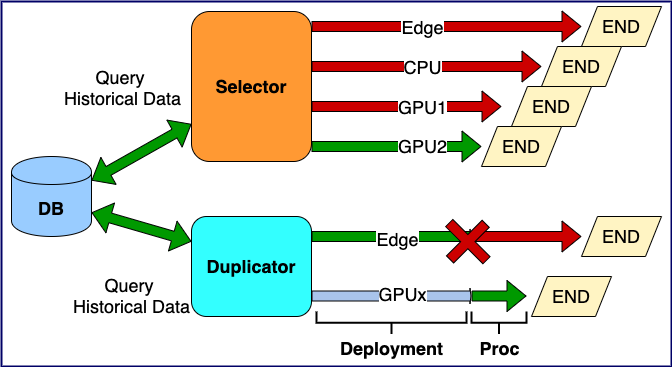
\includegraphics[scale=0.33]{figures/selector_duplicator.png}
\caption{The selector and duplicator modes of STOIC. 
\label{fig:duplicator}}
\end{figure}

The STOIC workflow is as follows: based on the three time components, STOIC
predicts the total response times~($T_s$) of the four deployment options. As
in the basic \textbf{selector} mode, the scheduler selects the runtime with
the shortest estimated response time. Seen in Figure~\ref{fig:duplicator}, the
edge cloud then schedules only one request, including the payload of
compressed image batch and runtime information. Upon execution, the edge cloud
triggers the serverless function locally if the choice is the \textit{edge}
runtime. Such deployment is common when a batch of images is small. 

For large batch sizes, STOIC typically schedules one of the three public
runtime options. For these three scenarios, the edge cloud first requests the
deployment on the public cloud. It then sends the payload to public cloud
storage. The public cloud then deploys the runtime on nodes that satisfy the
node affinity configuration. To handle unforeseen deployment failure, we
implement retry mechanism using exponential back-off delays. Starting at 100
milliseconds, STOIC waits 2X length of time for retrying the deployment on
Nautilus. After 10 failed attempts, STOIC claims timeout and returns an error.
From our experiments, this mechanism greatly reduces manual intervention and
successfully deploys most runtime in a timely manner.
 
Once Nautilus successfully deploys the serverless function, it informs the
edge cloud's requester to trigger the function via an HTTP request. To cope
with the cold starts~\cite{ref:coldstart}, STOIC triggers the function with
the least amount of input data to ensure the function caches the model in
memory. When the task completes, the requester retrieves the results and
runtime metrics, and transmits them back to the edge controller. Finally, the
edge cloud logs the results and metrics to the database for use in later
predictions. 

We observe from Table~\ref{tab:timeline} that the unstable deployment time of
GPU runtimes significantly affects the accuracy of prediction made by STOIC.
To address the issue, we reconfigure STOIC into the \textbf{duplicator} mode
demonstrated in Figure~\ref{fig:duplicator}. Based on the historical data, the
duplicator runs workload on edge cloud and GPU runtimes concurrently, and
halts the edge cloud execution if the remaining time at edge cloud is longer
than the expected processing time ($T_p$) at the GPU runtime once it completes
deployment. This ``lagging decision'' mechanism reduces the variability of
deployment time in the prediction. STOIC only has to consider processing time,
which is more accurately predicted, to deploy tasks. Note that duplicator is
less energy-efficient because it runs tasks regardless of latency prediction
and may waste cloud resources by killing the function in the middle. 

In addition, the inquisitor running in background deploys all runtime
scenarios on the public cloud and logs deployment time in the database for
prediction. We set a timeout (i.e. 10 minutes) for unresponsive nodes. That
is, inquisitor marks the runtime unavailable when the deployment hits the set
timeout. Instead of ignoring such runtime, the inquisitor keeps requesting all
runtimes across public cloud and resume the runtime's availability if the
following deployment is successful.

A final component is the regression initiator which performs bootstrapping.
Extended from the initial version, we enable STOIC to take application name
and versioning information as input. Once a new application is deployed or the
existing application is updated, the regression initiator automatically
executes two tasks based on the current application and version for each
runtime scenario. These two data points initialize the incoming regressions
and predictions across the edge and public cloud.

